\documentclass[tikz]{standalone}

\usepackage{xcolor}
\definecolor{morange}{RGB}{255,127,14}
\definecolor{mblue}{RGB}{31,119,180}
\definecolor{mred}{RGB}{214,39,40}
\definecolor{mpurple}{RGB}{148,103,189}
\definecolor{mgreen}{RGB}{44,160,44}

\usepackage{mathtools}
\usepackage{amssymb}  
\usepackage{nicematrix} 

\usepackage{tikz}
\usetikzlibrary{fit,shapes.geometric}
\tikzset{highlight/.style={rectangle, draw=mblue, semithick, inner sep=1pt}}

\begin{document}

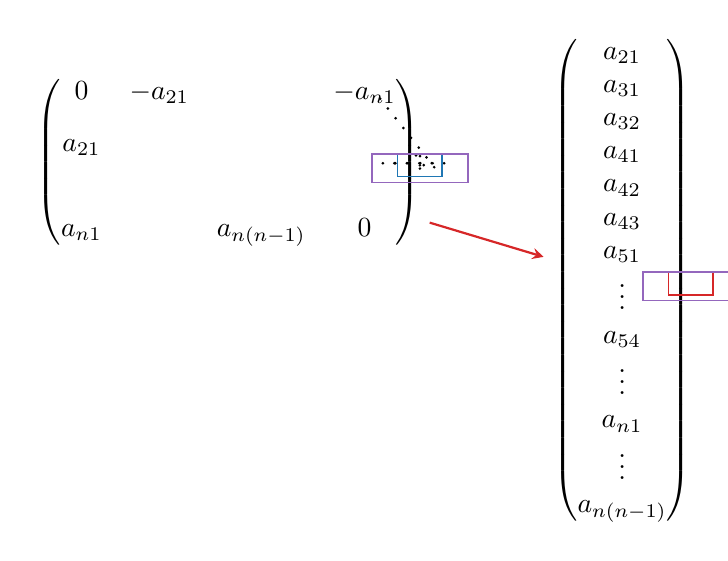
\begin{tikzpicture}

\node (matrix) {$
\begin{pNiceMatrix}[name=A]
     0 & -a_{21} & \Cdots & -a_{n1}      \\
     a_{21} & \Ddots &        & \Vdots \\
     \Vdots & \Ddots & \Ddots & \Vdots \\
     a_{n1} & \Cdots & a_{n(n-1)}      & 0 
     \CodeAfter
     \tikz \node [highlight, fit=(2-1)(2-1), mblue] {};
     %\tikz \node [highlight, fit=(2-1) (2-1), mpurple] {};
     \tikz \node [highlight, fit=(4-1)(4-3), mpurple] {};
\end{pNiceMatrix}
$};

\node[below of=matrix, xshift=5cm, yshift=-.5cm] (vector) {$
\begin{pNiceMatrix}
     a_{21} \\
     a_{31} \\
     a_{32} \\
     a_{41} \\ 
     a_{42} \\
     a_{43} \\
     a_{51} \\ 
     \vdots \\ 
     a_{54} \\ 
    \vdots \\
    a_{n1} \\ 
    \vdots \\
    a_{n(n-1)} 
    \CodeAfter
    \tikz \node [highlight, fit=(1-1)(1-1), mblue] {};
    \tikz \node [highlight, fit=(2-1)(3-1), morange] {};
    \tikz \node [highlight, fit=(4-1)(6-1), mgreen] {};
    \tikz \node [highlight, fit=(7-1)(9-1), mred] {};
    \tikz \node [highlight, fit=(11-1)(13-1), mpurple] {};
\end{pNiceMatrix}
$};

\draw[-stealth, thick, rounded corners, mred] (matrix) -- (vector);

\end{tikzpicture}
\end{document}

\end{document}